% --------------------------------------------------------------------------------

\begin{exercise}

Manufacturing and selling drugs that claim to reduce an individual's cholesterol level is big business.
A company would like to market their drug to women if their cholesterol is in the top $15 \%$.
Assume the cholesterol levels of adult American women can be described by a Normal model with a mean of $188 \text{mg / dL}$ and a standard deviation of $24 \text{mg / dL}$.

\begin{enumerate}[label = (\alph*)]

    \item Use \texttt R to draw and label the Normal model.
    
    \item What percent of adult women do you expect to have cholesterol levels over $200 \text{mg / dL}$?
    
    \item What percent of adult women do you expect to have cholesterol levels between $150 \text{mg / dL}$ and $170 \text{mg / dL}$?
    
    \item Calculate the interquartile range of the cholesterol levels.
    Recall, the interquartile range is the difference between upper and lower quartile, i.e.

    \begin{align*}
        \mathrm{IQR} = x_{0.75} - x_{0.25}.
    \end{align*}

    \item Above what value are the highest $15 \%$ of women's cholesterol levels?

\end{enumerate}

\textit{Hint:}
If using \texttt R for all computations the following commands \texttt{pnorm()}, \texttt{qnorm()} and \texttt{dnorm()} are useful.
Otherwise values from the table of the standard Normal distribution shold be used.

\end{exercise}

% --------------------------------------------------------------------------------

\begin{solution}

Let $X \sim N(188, 24^2)$ be the cholesterol level of an adult American woman (in $\text{mg / dL}$).

\begin{align*}
    g(x) := \frac{x - 188}{24},
    \quad
    Z := g(X) \sim N(0, 1)
\end{align*}

\begin{enumerate}[label = (\alph*)]

    \item 
    
    \lstset{style = fundament}
    \lstinputlisting{2.5.r}
    
    \begin{figure}[H]
        \centering
        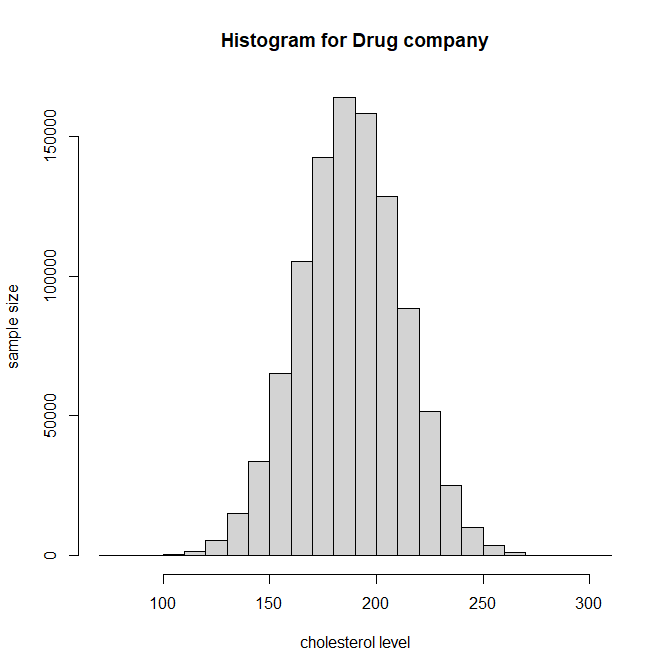
\includegraphics[width = 0.75 \textwidth]{2.5.png}
    \end{figure}

    \item

    \begin{align*}
        g(200) = 0.5
    \end{align*}

    \begin{align*}
        P(X > 200)
        =
        1 - P(X \leq 200)
        =
        1 - P(Z \leq 0.5)
        =
        1 - \Phi(0.5)
        \approx
        1 - 0.6915
        =
        0.3085
    \end{align*}

    \item

    \begin{align*}
        g(150) = -1.58 \dot 3,
        \quad
        g(170) = -0.75
    \end{align*}

    \begin{align*}
        P(150 < X < 170)
        & =
        P(X \leq 170) - P(X \leq 150) \\
        & =
        P(Z \leq -0.75) - P(T \leq -1.58 \dot 3) \\
        & =
        \Phi(-0.75) - \Phi(-1.58 \dot 3) \\
        & =
        (1 - \Phi(0.75)) - (1 - \Phi(1.58 \dot 3)) \\
        & =
        \Phi(1.58 \dot 3) - \Phi(0.75)
        \approx
        0.9429 - 0.7734 \\
        & =
        0.1695
    \end{align*}

    \item

    \begin{align*}
        &
        \Bbraces{0.25, 0.75} \ni p = P(X \leq x_p) = P(Z \leq g(x_p)) = \Phi(g(x_p)) = 1 - \Phi(-g(x_p)) \\
        \implies &
        x_{0.75} = g^{-1}(\Phi^{-1}(0.75))  \in  24 \cdot (0.67, 0.68) + 188 = (204.08, 204.32), \\
        &
        x_{0.25} = g^{-1}(-\Phi^{-1}(1 - 0.25)) \in -24 \cdot (0.67, 0.68) + 188 = (171.68, 171.92) \\
        \implies &
        x_{0.75} - x_{0.25} \in (32.16, 32.64)
    \end{align*}

    \item

    \begin{align*}
        x_{1 - 0.15}
        =
        x_{0.85}
        =
        g^{-1}(\Phi^{-1}(0.85))
        \in
        24 \cdot (1.03, 1.04) + 188
        =
        (212.72, 212.96)
    \end{align*}

\end{enumerate}


\end{solution}

% --------------------------------------------------------------------------------
